\section{Methodology}

\subsection{Description of the data}
% Data verzameling en beschrijving van de data
% Hoe is de data verzameld, en hoe heb jij die data verkregen?
% Wat staat er in de data? Niet alleen maar een technisch verhaal, maar ook inhoudelijk. DE lezer moet een goed idee krijgen over de technische inhoud en wat het betekent.
For classifying fake news, Wang's Liar dataset will be used \cite{wang2018}. 
The Liar dataset contains 12.791 short statements from Politifact.com, which are labeled manually by a Politifact.com editor on truthfulness. 
The statements are an average of 18 tokens long, and the topics vary from different political subjects, as can be seen in figure 1\todo{Check whether this number is still correct}.
Truthfulness is evaluated by assigning one of 6 labels, ranging from \textit{pants-on-fire} to \textit{true}. 
The distribution of statements across labels can be seen in figure X\todo{Create a figure comparing distributions of labels before and after preprocessing and insert the right figure number}. 

\begin{figure}[h]
    \centering
    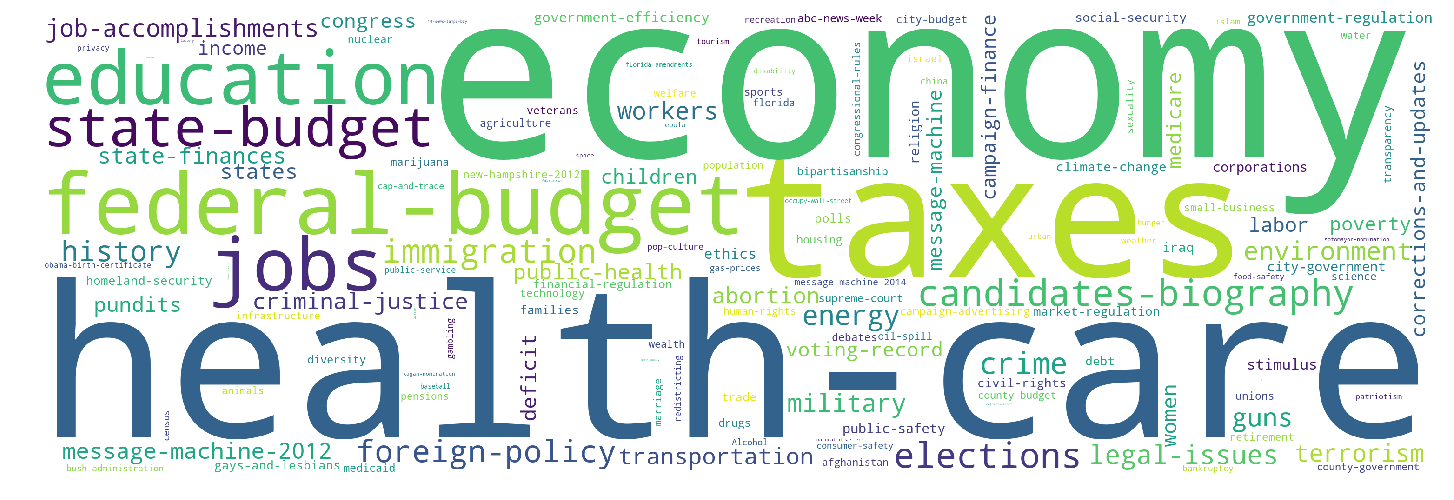
\includegraphics[scale=0.25]{subjectwordcloud}
    \caption{An overview of all statement topics in the Liar dataset.}
\end{figure}

For each statement, the dataset contains an id, a label, a subject, a speaker, the function title of the speaker, the affiliated state and political affiliation, the context of the statement and a vector with a truthfulness history.
Wang introduced this truthfulness history to boost the prediction scores, as speakers with a track record of lying are expected to have a lower chance of speaking the truth when classifying new statements.
However, for our application we are only interested in the statement itself and its corresponding label. 
Due to cheapness and spreadability, a large amount of fake news is spread over social media \cite{shu2017}. 
This means author information and metadata will not readily be available in real world circumstances.

The original dataset has been split beforehand into a test, train and validation set. 
The train set contains 80\% of the total amount of statements, while the test and validation set both contain approximately 10\% of the statements. 

\begin{figure}[h]
    \centering
    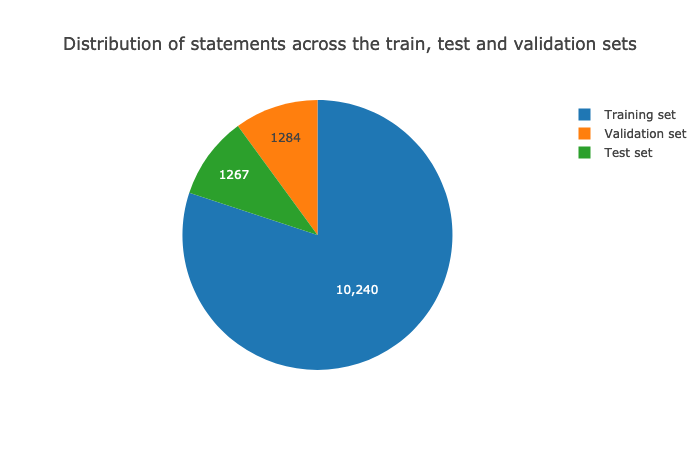
\includegraphics[scale=0.5]{folddistribution}
    \caption{Distribution of the total dataset.}
\end{figure}


\subsection{Data}
% Plotjes

\subsection{Methods}
% Hoe je je vraag gaat beantwoorden.
% Dit is de langste sectie van je scriptie. 
% Als iets erg technisch wordt kan je een deel naar de Appendix verplaatsen. 
% Probeer er een lopend verhaal van te maken.
% Het is heel handig dit ook weer op te delen nav je deelvragen:

\subsubsection{RQ1}

\subsubsection{RQ2}

\subsubsection{RQ3}
